% ==================================================================================================
% CHAPTER 5 -- RETRIEVAL (RQ1).  One file; content.tex inputs it directly.  There are no _secNN
% files: they were merged away 2026-09-21 and no longer exist.
%
% AUTHORITY.  thesis/manifest.md decides structure, research questions, hypotheses, decision rules
%   and every number -- §1b RQs, §1c hypotheses, §4 and §4c the chapter map and renumbering, §9 this
%   chapter's blueprint and page budget, §14 the experiment registry, §15 what is open.  CLAUDE.md
%   decides house style.  Nothing is restated here; where a note below cites one, read it there.
%
% SHAPE (manifest §4a).  5.1 overview -> 5.2 method -> 5.3 guards -> 5.4 results -> 5.5 the
%   containment diagnostic -> 5.6 verdicts.  §5.3 and §5.5 RULE ON NO HYPOTHESIS: §5.3 answers two
%   threats, §5.5 explains §5.4's result and therefore follows it.
%
% HEADING DEPTH (manifest §4b).  tocdepth is 2, so a \subsubsection is numbered but never appears in
%   the table of contents.  Inside §5.4 each experiment is continuous argument with bold run-in
%   lead-ins and NO numbered subheadings; §5.3's two guards and §5.5 follow the same rule.  Never
%   raise tocdepth to work around this.
%
% STANDING RULES THAT BITE HERE (manifest §1c-i and §9; CLAUDE.md §4):
%   - nDCG' and P' at @5/@10/@20 only.  @100 and @1000 appear nowhere.  ndcg'@10 is primary and
%     every decision rule reads it.  bpref and retrieval recall are reported nowhere.  MAP' appears
%     in exactly two places in the thesis: §4.3 calibration and §5.3's formula-search guard.
%   - §5.4 reports the JUDGE labels only.  The assessors' labels and the hole rates appear once, in
%     §5.3.  No hole or fill column in §5.4 -- under the judge pool it is zero by construction.
%   - 78 official topics for answer retrieval (qrel_task1_2022_official.tsv), macro average; never
%     the 87 or the 100.  Formula search keeps its own official qrels, 76 topics.
%   - No significance testing, no interval, and the word "significant" nowhere.  A difference of
%     0.02 or less between values AS PRINTED is indistinguishable (R4.4, §4.4; manifest §15 O-19 b).
%   - No comparison with published answer-retrieval systems.  The formula-search comparison against
%     TangentCFT2 stays, in §5.3, as the component guard -- §1c-i decision 3 exempts it.
%   - Never write a number the registry (manifest §14) does not contain.  If one is missing, say so.
%
% TERMINOLOGY.  "answer retrieval" and "formula search", never a bare task number -- §3.1 grounds
%   both terms and §4.2 grounds formula search again, so no ARQMath task number appears anywhere in
%   this chapter.  "formulas", not "formulae".  No "channel" (retired, manifest §15 O-14): index for
%   the thing, retrieval for the act, judge labels and assessors' labels for the two label sets.
%   Coined terms are defined at first use -- fanout, trivial, formula block, blocked, flat and
%   leave-one-out in §5.2.2, judge pool in §5.2.3.  There is no notation table (§15 O-14).
%
% FLOATS -- READ BEFORE CHANGING ANY TABLE.  Tables are placed in declaration order, so ONE table
%   that cannot be placed defers EVERY later table in the chapter, and it fails silently: nothing
%   appears in the log, the tables simply turn up pages later, often past the chapter end.  Figures
%   queue separately, so figures sitting correctly proves nothing about the tables.  The class sets
%   no float parameters, so LaTeX defaults apply (\topfraction 0.7, \textfraction 0.2, totalnumber
%   3).  This happened on 2026-09-25: tab:met-fusion grew and Tables 5.3-5.8 all flushed onto pages
%   62-65, inside Chapter 6.  Fixed with [!t] on that one float.  AFTER GROWING A TABLE OR MOVING A
%   CAPTION, check where every later table lands by reading the \newlabel page numbers in
%   ausarbeitung.aux -- not by scrolling the PDF.
%
% CAPTIONS.  Every caption sits BELOW its tabular with the \label immediately AFTER the caption, and
%   stands alone with every abbreviation expanded (reviews C4 and E3; manifest §15 O-8).  A \label
%   placed above its \caption silently picks up the section counter instead of the table number.
%
% BUILD.  Abram builds and reads the log.  Do not compile from here, and leave *.aux, *.log, *.pdf
%   and the other artefacts alone.  Verify references by grep, not by compiling.
%
% CHANGELOG 2026-09-25 -- every part drafted in the chat and approved before the write (CLAUDE.md §2
%   steps 5-6).  §5.4 rewritten into six subsections; §5.5 cut to the one-page diagnostic; §5.6
%   rewritten against the 2026-09-24 hypothesis set; §5.1 rewritten with its RQ block and mapping
%   table deleted; §5.2 tightened end to end; §5.3 rewritten as "Guards"; Tables 5.3-5.5 captions
%   cut; the float dam fixed.  Closes manifest §15 O-21 in full, O-20 (c), O-19 (a) and (e), and
%   O-17 (iv).  Swept to zero across all six sections: bare task numbers, "matters most" ranking
%   clauses (review E4), retired hypothesis IDs, "formulae", "channel", "significant", @100/@1000.
% ==================================================================================================
\chapter{Retrieval}\label{ch:retrieval}


% §5.1 OVERVIEW -- rewritten 2026-09-25 (manifest §9 row 5.1; closes §15 O-20 (c)).
% The RQ block and the experiment->RQ->hypothesis table (tab:ret-overview) were DELETED rather than
%   restated to the current wording: both had gone stale twice, and the mapping is already carried
%   by §5.4.1's overview, by each results subsection's opening sentence and by §5.6's one-to-one
%   verdicts.  Manifest §4a's "§5.1 carries the mapping table" lapsed with it, and §6.1 follows the
%   same shape.  tab:ret-overview was referenced only from inside §5.1, so nothing dangles.
% Kept here and NOWHERE ELSE: ndcg'@10 named as the primary measure -- §5.6 reads "the primary
%   measure" three times against this sentence.  The 0.02 reading rule is restated here on Abram's
%   decision although §4.4 also states it in full; §5.2.3 back-references this section for the
%   judge's generous grading, so the paragraph has to stay.
% Does not use "configuration": the term is defined in §5.2.2, its natural home.
\section{Overview}\label{sec:ret-overview}

This chapter answers the first research question, on retrieval, posed in
Section~\ref{sec:intro-rqs}. Section~\ref{sec:ret-method} builds the systems it compares and
fixes what they are scored against. Section~\ref{sec:ret-guards} answers two threats to those
scores before any of them is read: that the formula index does not work at all, and that the
ARQMath assessors' labels do not cover what these systems retrieve.
Sections~\ref{sec:ret-results} and~\ref{sec:res-transfer} report and explain the results, and
Section~\ref{sec:ret-verdicts} rules on each hypothesis.

The measures reported are nDCG$'$ and P$'$ at cutoffs 5, 10 and 20. nDCG$'$@10 is the primary
measure, and every decision rule that compares answer-retrieval rankings reads it. Where a rule
reads more than that, the section applying it says so. The other two cutoffs show the shape of a
ranking and decide nothing.

The answer-retrieval values compare retrieval systems with one another; they are not benchmark
figures. They are computed against the labels of the relevance judge of
Section~\ref{sec:met-judge-validation}, which grades more generously than the ARQMath assessors,
so no comparison with published systems for the task is made. Differences are read under that
section's rule: a difference of 0.02 or less between the values as reported is indistinguishable.


% §5.2 METHOD -- opener.  Opens from what Chapters 3 and 4 established and says what is left for
%   retrieval alone (CLAUDE.md §3a).  States no outcome and uses no coined vocabulary.
% §5.2.3 is introduced as FIXING the evaluation pipeline, not validating it.  Validation is Chapter
%   4's: P1 is §4.3's calibration, P2 is §4.4's judge validation.  The word "validates" stood here
%   briefly on 2026-09-25 and was corrected the same day -- it promised evidence §5.2 does not carry
%   and read as a guard inside a method section, which CLAUDE.md §3a forbids.  Keep the distinction
%   when §6.2 is written.
\section{Method}\label{sec:ret-method}

Section~\ref{sec:ret-overview} fixed how this chapter's numbers are read. That reading
holds only if every ranking was produced as described and every answer-retrieval ranking was
scored against the same judgments, so this section states how the rankings were produced and what
they are scored against. Chapter~\ref{ch:background} defined the formula representations,
the three families of retrieval, rank fusion and the prime measures.
Chapter~\ref{ch:setup} placed the indices in the system in
Section~\ref{sec:met-system-overview}, fixed how a ranking is scored in
Section~\ref{sec:met-calibration}, and validated the judge that labels it in
Section~\ref{sec:met-judge-validation}. What remains is what retrieval alone needs.
Section~\ref{sec:met-formula-indexing} builds the formula indices.
Section~\ref{sec:met-retrieval-configs} turns a topic into queries and fixes the fusions
compared. Section~\ref{sec:met-evaluation-protocol} fixes the evaluation pipeline: every
answer-retrieval effectiveness figure in
Section~\ref{sec:ret-results}, and the retrieval quality Chapter~\ref{ch:generation}
reads, is computed against the judgments it assembles.

% §5.2.1 FORMULA REPRESENTATION AND INDEXING -- rewritten 2026-09-20.
% Opens from §3.2 (trees, tuples, the window) and §3.3 (fastText, approximate search) and redefines
%   neither: no tuple positions, no mean-of-tuples definition, no IVF mechanism.
% tab:met-tuples is the thesis's one full tuple table -- Table 3.1 was deleted 2026-09-20 and §3.2
%   now defines the window without a value.  Tuples checked against the extractor,
%   get_pairs(window=2, eob=True), on the organisers' MathML for collection formula 26878010
%   (x-y^2=0): 11 SLT, 14 OPT; a window of 1 gives 7 and 10.
% Topic formulas are converted with latexmlmath at query time in BOTH tasks -- formula_selector.py,
%   faiss_scalar_quantizer.py _generate_query_embedding, task2_formula_retrieval.py embed_query --
%   not read from _representation_v3.
% Indexing, as the code does it: the answer-retrieval indices (faiss_scalar_quantizer.py) hold the
%   raw mean vectors and search by FAISS's default squared L2; the formula-search index
%   (build_collection_formula_index.py) centres on the vocabulary mean and scales to unit length,
%   i.e. cosine.  Both are stated plainly and without comment -- manifest §15 O-16.
% Tuple position [3] is included in the encoding: confirmed by Abram from the code, 2026-09-20
%   (manifest §12 L1).  fastText settings are Tangent-CFT's reported SLT/OPT ones (300, 3-6,
%   skip-gram, 20, window 5); epochs 5 is gensim's default and min_count 1 (formula_model_manager.py),
%   where Tangent-CFT's released config trains for 30 -- stated in the prose.
\subsection{Formula representation and indexing}\label{sec:met-formula-indexing}

Section~\ref{sec:bg-formula-representations} defined the three tree representations, the
path tuples derived from them and the window that bounds a tuple, and
Section~\ref{sec:bg-indexing} how a sequence of tuples becomes a vector that can be searched.
This section states how that was done here: where the trees come from, how the tuples are
encoded and embedded, and how the vectors are indexed. The tuples are all the index ever sees
of a formula: two formulas can be found similar only through the tuples, and the parts of
tuples, that they share.

The implementation adapts the released code of
Tangent-CFT~\cite{mansouri2019tangentcft}\footnote{\url{https://github.com/BehroozMansouri/TangentCFT}}
for parsing trees, extracting tuples and encoding them for fastText, and departs from it in
three places. The trees of the collection's formulas are read from the organisers' MathML
rather than converted from \LaTeX{}. Each representation has an index of its own rather than
contributing to a single vector summed across the three. And the vectors are searched with an
approximate nearest-neighbour index, where Tangent-CFT holds every formula vector in memory
and compares the query with each of them.

\textbf{Trees and tuples.} The MathML of every formula in the collection is read from the
organisers' \texttt{latex}, \texttt{slt} and \texttt{opt} \texttt{\_representation\_v3}
files. These key each formula by its identifier and record its visual identifier, its post
and the post's type, and they are the corrected representations released for
ARQMath-3~\cite{mansouri2022arqmath3}. A topic's formulas are converted from their \LaTeX{}
with LaTeXML~\cite{millerlatexml} when the topic is queried, in both tasks. Each tree is
traversed with end-of-baseline markers and a window of two, Tangent-CFT's
setting~\cite{mansouri2019tangentcft}. Table~\ref{tab:met-tuples} gives every tuple this
produces for $x - y^2 = 0$: eleven in the SLT and fourteen in the OPT, four of each joining
nodes two edges apart. A window of one would give seven and ten.

\begin{table}[t]
\centering
\begin{tabular}{@{}ll@{}}
\toprule
\textbf{SLT tuples} & \textbf{OPT tuples} \\
\midrule
\ttfamily (V!x, -, n, -)              & \ttfamily (U!eq, O!minus, 0, -) \\
\ttfamily (V!x, V!y, nn, -)$^\dagger$ & \ttfamily (U!eq, O!SUP, 01, -)$^\dagger$ \\
\ttfamily (-, V!y, n, n)              & \ttfamily (U!eq, V!x, 00, -)$^\dagger$ \\
\ttfamily (-, N!2, na, n)$^\dagger$   & \ttfamily (O!minus, V!x, 0, 0) \\
\ttfamily (-, =, nn, n)$^\dagger$     & \ttfamily (V!x, 0!, 0, 00) \\
\ttfamily (V!y, N!2, a, nn)           & \ttfamily (O!minus, O!SUP, 1, 0) \\
\ttfamily (N!2, 0!, n, nna)           & \ttfamily (O!minus, N!2, 11, 0)$^\dagger$ \\
\ttfamily (V!y, =, n, nn)             & \ttfamily (O!minus, V!y, 10, 0)$^\dagger$ \\
\ttfamily (V!y, N!0, nn, nn)$^\dagger$ & \ttfamily (O!SUP, V!y, 0, 01) \\
\ttfamily (=, N!0, n, nnn)            & \ttfamily (V!y, 0!, 0, 010) \\
\ttfamily (N!0, 0!, n, nnnn)          & \ttfamily (O!SUP, N!2, 1, 01) \\
                                      & \ttfamily (N!2, 0!, 0, 011) \\
                                      & \ttfamily (U!eq, N!0, 0, -) \\
                                      & \ttfamily (N!0, 0!, 0, 0) \\
\bottomrule
\end{tabular}
\caption[Tuples extracted from a worked formula]{Every tuple extracted from $x - y^2 = 0$ with a window of two, in the symbol layout
tree (SLT) and the operator tree (OPT). Each tuple reads (node, descendant, edge labels on
the path between them, path from the root to the first node). Tuples marked $\dagger$ join
nodes two edges apart; a window of one produces only the others. \texttt{0!} marks the end
of a baseline in the SLT and a leaf in the OPT.}
\label{tab:met-tuples}
\end{table}

\textbf{Encoding.} Each tuple becomes one word for fastText. Following Tangent-CFT, a node
label is split into its type and its value, so \texttt{N!2} contributes the two tokens
\texttt{N!} and \texttt{2}. Edge labels get identifiers of their own, so a relation can never
be confused with a symbol. Every token is written as a single Unicode character, with node
tokens numbered from 60{,}000 and edge tokens from 500. A tuple therefore becomes a short
string with one character per component, and each of fastText's character n-grams is a run of
whole components. The tuples of $y^2$ and of $z^2$ at the same position,
\texttt{(V!y, N!2, a, nn)} and \texttt{(V!z, N!2, a, nn)}, are different words, but they share
every n-gram that does not include the variable, so their vectors lie close together.
SLT-TYPE needs no tree of its own: it is the SLT's tuples encoded with every value dropped, so
\texttt{N!2} contributes \texttt{N!} alone.

Position \texttt{[3]}, the path from the root, is encoded as part of the word. Tangent-CFT
omits it, judging that it may mislead the embedding, particularly in the OPT, where it is only
a sequence of argument positions~\cite{mansouri2019tangentcft}. It is kept here, because
without it a pair near the root of one formula and the same pair deep inside another become
the same word, so two formulas share vocabulary they do not share structurally. The
alternative was not run.

\textbf{Embedding.} One fastText model per representation is trained with
gensim~\cite{rehurek2010gensim} over the encoded tuples of the collection's formulas. The
settings in Table~\ref{tab:met-fasttext} are those Tangent-CFT reports for its SLT and OPT
models~\cite{mansouri2019tangentcft}, applied here to all three representations. The one
difference is the number of epochs, which the paper does not give: Tangent-CFT's released
configuration trains for thirty, and the models here were trained for five, gensim's default.

\begin{table}[t]
\centering
\begin{tabular}{ll}
\toprule
Setting & Value \\
\midrule
Vector size       & 300 \\
Character n-grams & length 3 to 6 \\
Objective         & skip-gram \\
Negative samples  & 20 \\
Context window    & 5 tuples either side \\
Epochs            & 5 \\
Minimum count     & 1 (every tuple kept) \\
\bottomrule
\end{tabular}
\caption[fastText settings for the tuple embeddings]{fastText settings used to train the tuple embeddings, identical for the symbol layout
tree (SLT), the operator tree (OPT) and SLT-TYPE, the SLT with its values erased. The context
window counts neighbouring tuples in a formula's tuple sequence, not edges in its tree.}
\label{tab:met-fasttext}
\end{table}

\textbf{Indexing.} Each representation's vectors are indexed with
FAISS~\cite{johnson2021faiss} as an inverted file with scalar quantisation. The index has
16{,}384 cells and scans the 256 nearest the query; every vector is stored in half precision,
and the cells are learned from a sample of the vectors. The answer-retrieval indices cover the
formulas of the answer posts. Each indexed vector keeps the identifiers of its formula and of
the answer it occurs in, so a hit on a formula is a hit on that answer. The formula vectors are
indexed as they are and searched by squared Euclidean distance. The formula-search index covers
every formula in the collection, in questions as well as answers. Each of its vectors is centred by
subtracting the average tuple vector and then scaled to length one, and the query is treated
the same way. For vectors of length one, Euclidean distance ranks formulas in the same order
as cosine similarity.

The index answers one formula at a time, while a topic is a question holding several. Which
of them are sent to the index, and how their hits become one ranking of answers, is the first
thing Section~\ref{sec:met-retrieval-configs} settles.

% §5.2.2 RETRIEVAL CONFIGURATIONS -- rewritten 2026-09-20, tightened 2026-09-25.
% Defines configuration, fanout, trivial, formula block, blocked, flat and leave-one-out BEFORE the
%   fusion table (review C3 asked for the triviality filter with a worked example before first use).
%   Fanout with the triviality filter on is stated as THE METHOD, justified a priori (manifest §4e);
%   the heuristic and filter-off variants are not reported anywhere and their runs stay in the
%   registry (closed item §15 O-5).
% Naming BM25 and SLT-TYPE as the weakest of their kind rests on the single-index results: the one
%   deliberate forward reference from a method section to a result (manifest §4e).
% Code: formula_selector.py (select_fanout, is_trivial -- OPT prefixes O!/U!/F!/+!/M! non-trivial,
%   V!/N!/C!/T! content); metrics.py generate_run_file (a reciprocal-rank sum over formula HITS,
%   several per answer possible -- NOT RRF over answers); fuse_runs.py (RRF over stored runs,
%   k = 60); run_task2_experiment.py (instance-level RRF, collapse to visual ids, the query's own
%   visual id excluded).  x^n -> O!SUP via LaTeXML's "superscript" csymbol (semantic_symbol.py).
% 2026-09-25: the two fusion-design paragraphs collapsed into one and their reasons moved into
%   tab:met-fusion's group rows; RQ1.3 dropped from the "chosen to answer" clause (retired, manifest
%   §1b); and "which also gives a second blocked--flat comparison, without BM25" deleted -- H1.3's
%   rule reads the two full systems only since that day, so §5.4.5 never makes that comparison
%   (manifest §15 O-19 c).
% Open items from the 2026-09-20 rewrite: manifest §15 O-17.
\subsection{Retrieval configurations}\label{sec:met-retrieval-configs}

Section~\ref{sec:bg-indexing} described three families of retrieval, each returning a ranked
list on a scale of its own, and Section~\ref{sec:bg-rank-fusion} a way of combining such lists
that never compares their scores. Section~\ref{sec:met-formula-indexing} built the formula
indices but left one question open: a topic is a question holding several formulas, and a
formula index answers one formula at a time. This section settles that question, states how a
topic is put to the sparse and dense indices, and fixes the fusions this chapter compares. The
same rankings can be combined in more than one way, and whether the way matters is one of the
questions Section~\ref{sec:res-fusion} answers.

The formula indices are queried by \emph{fanout}: every distinct formula of the topic that is
not trivial becomes a query of its own, so the system never has to decide which formula a
question is about. A formula is \emph{trivial} when it gives an index nothing to match on.
Triviality is judged on the formula's operator tree rather than on its \LaTeX{} string. A
formula is trivial when no tuples can be extracted from it, as happens for an extraction
artefact such as \texttt{a)}, or when its tree holds no operator, function or matrix node and
at most one distinct variable, number or constant. A bare set name such as $\mathbb{R}$ is
therefore trivial, while $x^n$ is not, since its tree has the superscript operator
\texttt{O!SUP} that Table~\ref{tab:met-tuples} shows for $y^2$. A test on string length would
get both wrong, keeping a long variable name and discarding a short equation. The test is
applied to the operator tree whichever index is queried, so all three formula indices receive
the same query formulas, and a topic whose formulas are all trivial is queried with the one
that has the most operator-tree tuples. Fanout and the triviality filter are the design choices
of this thesis, held fixed in every experiment.

Each query formula returns the 1{,}000 formulas closest to it, and every one of them counts
towards the answer it appears in. A formula counts for more the higher it is ranked: it adds
$1/(60 + r)$ to its answer's score, where $r$ is its rank in its query's list, which is the
reciprocal-rank weighting of Section~\ref{sec:bg-rank-fusion}. The answers are then ranked by
their totals, so an answer containing several formulas close to the question's rises above an
answer containing only one.

The sparse and dense indices are queried with the topic's text, its title and question as
parsed in Section~\ref{sec:met-collection}, with the formulas left in their \LaTeX{}. The
sparse index is built with Pyserini~\cite{lin2021pyserini}, the Python interface to Anserini,
which is built on Lucene, and scored by BM25 with that toolkit's default parameters, $k_1 = 0.9$ and
$b = 0.4$. The dense index holds one vector per answer post from
\texttt{multi-qa-\allowbreak mpnet-\allowbreak base-\allowbreak dot-v1}, a bi-encoder from the sentence-transformers
library~\cite{reimers2019sbert}, built on the MPNet language model~\cite{song2020mpnet} and
fine-tuned on question--answer pairs. The topic text is encoded with the same model and
compared by dot product with every stored vector, so the dense index is searched exhaustively
where the formula indices are searched approximately. The encoder is used as published, with no
further training on mathematical text.

Each index returns at most 1{,}000 answers per topic, so every topic yields five ranked lists of
answer posts: BM25, dense, and one for each formula representation. Each list is stored as a
run, and every fusion reads the stored runs rather than querying an index again, so a fused list
can be rebuilt from the runs it combines. A retrieval \emph{configuration} is a choice of which
of these rankings are used and, where there is more than one, how they are combined. Fifteen
configurations are reported: each of the five rankings on its own, and the ten fusions of
Table~\ref{tab:met-fusion}.

Every fusion is reciprocal rank fusion with $k = 60$ over whole rankings of answers, so a
ranking contributes to an answer's score at most once; no score is normalised and no ranking is
weighted. The three formula rankings can enter a fusion in two ways, and the difference is the
point. Fused with one another, SLT, OPT and SLT-TYPE give a single ranking, the \emph{formula
block}. In a \emph{blocked} fusion the formula block enters beside the text rankings as one
input; in a \emph{flat} fusion the three formula rankings enter separately, each on the same
footing as BM25 and dense. Since reciprocal rank fusion weighs every input equally whatever it
retrieves, a flat fusion of all five hands three of the five votes to three views of the same
formulas, where a blocked fusion hands them one of three. A blocked configuration therefore
combines at three levels: the hits of each query formula within one representation, the three
representations within the block, and the block with the text rankings.

The ten fusions in Table~\ref{tab:met-fusion} answer the two sub-questions with few runs rather
than sweeping every combination, and they fall into five groups. Dense retrieval is the text side
in every pair, as the stronger of the two text indices in the single-index results of
Section~\ref{sec:res-single-index}, so that the text side is held fixed and any difference between
the three pairs comes from the representation. The last group removes one index from a full
system, a \emph{leave-one-out} ablation, and the index removed is the weakest of its kind on its
own: BM25 of the two text indices, and SLT-TYPE of the three formula indices, as those same
single-index results show. Reciprocal rank fusion gives a weak ranking the same vote as a strong
one, so if an index costs a fused system more than it adds, the weakest is the likeliest to.
SLT-TYPE is removed from the flat fusion only: there its ranking has a full vote, as much as dense
retrieval, while inside the blocked fusion it is only one of the three rankings that make up the
block.

% [!t], NOT [t].  See the FLOATS note in the chapter header: this float dammed the whole table
%   queue on 2026-09-25 and the ! is what clears it.  Kept even though the shorter caption now lets
%   it place under [t] as well -- the margin is thin and the failure is silent.
\begin{table}[!t]
\centering
\small
\renewcommand{\arraystretch}{1.2}
\begin{tabularx}{\textwidth}{@{}l>{\raggedright\arraybackslash}X@{}}
\toprule
Configuration & Rankings fused \\
\midrule
\multicolumn{2}{@{}p{\textwidth}@{}}{\emph{Text only --- the system the formula indices are added to}} \\
\addlinespace[0.2em]
BM25 + dense          & BM25, dense \\
\addlinespace[0.6em]
\multicolumn{2}{@{}p{\textwidth}@{}}{\emph{One formula index added --- the text side held fixed, so the representation is the only thing that changes}} \\
\addlinespace[0.2em]
dense + SLT           & dense, SLT \\
dense + OPT           & dense, OPT \\
dense + SLT-TYPE      & dense, SLT-TYPE \\
\addlinespace[0.6em]
\multicolumn{2}{@{}p{\textwidth}@{}}{\emph{Formula only --- the three formula rankings with no text}} \\
\addlinespace[0.2em]
formula block         & SLT, OPT, SLT-TYPE \\
\addlinespace[0.6em]
\multicolumn{2}{@{}p{\textwidth}@{}}{\emph{All three added --- the same five rankings, differing only in whether formula evidence enters as one input or as three}} \\
\addlinespace[0.2em]
blocked               & BM25, dense, formula block \\
flat                  & BM25, dense, SLT, OPT, SLT-TYPE \\
\addlinespace[0.6em]
\multicolumn{2}{@{}p{\textwidth}@{}}{\emph{One index removed --- if a system is worse without an index, that index was contributing}} \\
\addlinespace[0.2em]
blocked, $-$BM25      & dense, formula block \\
flat, $-$BM25         & dense, SLT, OPT, SLT-TYPE \\
flat, $-$SLT-TYPE     & BM25, dense, SLT, OPT \\
\bottomrule
\end{tabularx}
\caption[The ten fused configurations]{The ten fused configurations on answer retrieval, each a reciprocal rank fusion
($k = 60$) of the rankings listed. \emph{SLT}: symbol layout tree. \emph{OPT}: operator tree.
\emph{SLT-TYPE}: the SLT with its values erased, node types only. The \emph{formula block} is the
three formula rankings fused into one; a \emph{blocked} fusion takes it as a single input, a
\emph{flat} fusion takes the three separately. A minus sign marks the index removed.}
\label{tab:met-fusion}
\end{table}

At formula search the formula block is the only configuration, run over the collection-wide
index of Section~\ref{sec:met-formula-indexing}. A formula-search topic is a single formula, so
there is nothing to select: each representation returns the 1{,}000 formula instances nearest
the topic formula, the three lists are fused by reciprocal rank fusion with $k = 60$, and the
result is collapsed to the organisers' visual identifiers, keeping the highest-ranked instance
of each, before it is cut to 1{,}000. Instances sharing the topic formula's own visual
identifier are left out.

Every answer-retrieval configuration thus ends in one ranked list of answers per topic, fifteen
rankings of each topic in all. What those rankings are scored against --- which of their
answers carry a relevance label, from whom, and to what depth --- is the question
Section~\ref{sec:met-evaluation-protocol} settles.

% §5.2.3 EVALUATION PROTOCOL -- rewritten 2026-09-20 (manifest §9 row 5.2; §7a).
% Scope: which judgments every answer-retrieval ranking is scored against and how -- the labelling
%   depth, the judge pool, the order of operations, the shared ideal -- then what formula search is
%   scored against instead, and the two places the assessors' labels are read (§5.3 and §5.5).
% Numbers.  Judge pool: results/rearranged/judge_qrels_pooled/
%   qrel_task1_2022_official_judge_pool20.tsv -- 7,532 labelled pairs over 78 topics, 81-116 per
%   topic -- with excluded_unparsed.tsv (8 pairs); manifest §1c-ii.  Formula search:
%   data/raw/qrels/qrel_task2_2022_official.tsv -- 76 topics, 11,538 pairs (H 1,215, M 1,600,
%   L 1,990, N 6,733); manifest §9 row 5.2.
% NOT here: pytrec_eval, the grade as gain and the H+M threshold (§4.3); ndcg'@10 as primary and the
%   0.02 rule (§5.1); the per-run construction the pooled qrel replaced, or any number comparing the
%   two -- it was corrected before any reported figure, so it is not a finding (manifest §9 row 5.2);
%   the hole rates on these runs (§5.3).
% 2026-09-25: the closing paragraph now names §5.3 as holding TWO threats (manifest §15 O-21 i).
\subsection{Evaluation protocol}\label{sec:met-evaluation-protocol}

Section~\ref{sec:bg-retrieval-metrics} showed that the ideal nDCG divides by is computed
from a topic's judgments, not from the ranking being scored, so two nDCG values can be
compared only when both are computed against the same judgments. The fifteen rankings of
Section~\ref{sec:met-retrieval-configs} therefore need one set of judgments between them,
and the organisers' cannot be it: their judgments cover what the 2022 participants
retrieved, not what these rankings retrieve.
Section~\ref{sec:met-judge-validation} validated a language model as a relevance judge:
its labels put systems in the same order as the assessors' labels do, so it can supply
judgments for answers the assessors never saw. Which answers those are is settled here.
This section defines the set of answers the judge labels, how a ranking is scored against
that set, and what formula search is scored against instead. The set fixes the ideal every
answer-retrieval ranking is measured against.

Only the head of a ranking is labelled, because only the head is used: the generator of
Section~\ref{sec:met-system-overview} receives the top $k$ answers of a ranking and nothing
below them. Each ranking is labelled to rank 20. That covers the cutoffs of 5 and 10 and
leaves room to show how a ranking continues below them. Twenty is therefore also the
deepest cutoff reported: a measure reading further would reach answers the ranking was
never labelled for.

The labels are gathered by the pooling of Section~\ref{sec:bg-arqmath}, with the fifteen
configurations in place of the participants' runs and one depth, 20, for all of them. For
each of the 78 topics, the top 20 answers of every configuration are merged and
deduplicated, and each answer in the result is graded by the judge. That set of labels is
the \emph{judge pool}. No assessor's grade enters it, not even for an answer the organisers
judged, so that every label in it comes from one judge applying one scale. Fifteen rankings
of twenty answers could put at most 300 answers into a topic's pool; because the rankings
overlap, each topic's pool holds between 81 and 116 answers, 7{,}532 in all across the 78
topics. The judge's output for eight further answers could not be parsed, and those answers
are left unjudged.

A ranking is scored against the judge pool after being cut to its top 20 and then
condensed, as the prime measures require. Inside that top 20 every answer carries a label
but for any of those eight, so the results of Section~\ref{sec:ret-results} report no hole
rate.

Because every configuration is scored against the same judge pool, each topic has one
ideal, shared by all fifteen, and their nDCG$'$ values can be set beside one another. The
ideal is drawn from the pool alone, so it holds only what the fifteen configurations
retrieved: a relevant answer that none of them placed in its top 20 raises no topic's
ideal. That is the second reason, beside the judge's generous grading noted in
Section~\ref{sec:ret-overview}, why the answer-retrieval values compare configurations
with one another and are not benchmark figures.

Formula search is scored as the organisers scored it, because
Section~\ref{sec:guard-task2} sets the formula block beside a published system. The judgments
are theirs: 11{,}538 judged pairs of a topic and a visually distinct formula over 76 topics,
of which 1{,}215 are High, 1{,}600 Medium, 1{,}990 Low and 6{,}733 Not relevant. The measures
are ARQMath's own for the task, nDCG$'$ and MAP$'$ over the whole ranking with P$'$@10 beside
them. MAP$'$ appears here and in none of the answer-retrieval results, because it belongs to
the measure set the published figures are given in. No judge labels are used there: the judge
grades answers to a question, not formulas.

The organisers' judgments for answer retrieval are not set aside.
Section~\ref{sec:res-transfer} measures how far a topic's formulas appear inside the
answers the assessors judged relevant and inside those they judged not relevant; it
computes no retrieval measure, so the judge pool does not enter it.
And Section~\ref{sec:ret-guards} scores the same fifteen rankings against the judgments of
Table~\ref{tab:met-qrels} as the organisers scored their participants, condensing the full
ranking before the cutoff, and asks how much of these rankings those judgments leave unjudged
and what that does to the scores they give --- the second of the two threats that section
takes up.


% §5.3 GUARDS -- rewritten 2026-09-25, closing manifest §15 O-21 (i), the last of that item.
% TWO guards, both as bold lead-ins rather than \subsubsection (§4b), under a section opener stating
%   what a guard answers here and that NEITHER RULES ON A HYPOTHESIS (manifest §4a).
%   "Formula search" -- the component guard: the index might simply be broken.  Answerable before
%     any answer-retrieval result exists, which is why it comes first; that is the answer to review
%     E7's worry about experiment order, and it is her own A5.  Single site of the TangentCFT2
%     comparison, which §1c-i decision 3 exempts from the no-published-comparison rule.
%   "Hole rates under the ARQMath labels" -- the coverage guard: the labels might not cover what
%     these systems retrieve.  Single home of claim C-4 (manifest §3).  @10 only and no P' at all
%     (Abram, 2026-09-20): it compares two scoring conventions on one cutoff, not a ranking's shape.
% Both guards previously opened on RQ1.1 and H1.1 (a), retired 2026-09-24 (manifest §1c migration
%   table); each now opens on its threat.  Both handoffs were also wrong before this rewrite -- the
%   first handed past the guard beside it, the second promised an experiment that now sits above it.
% Numbers.  Formula search: this thesis 0.615 / 0.420 / 0.592 with hole@10 0.355; TangentCFT2
%   0.641 / 0.419 / 0.534 with hole@10 0.026, its scores from the lab overview Table 4 and its hole
%   rate measured here from its submitted run.  Recovery 1,715 of 2,815 (manifest §14 R5); pool
%   density 2,815 of 11,538 against 2,943 of 34,847.  Hole table:
%   results/rearranged/metrics_human_only/metrics_aggregate.csv, 78 topics, macro average.
%   Corrected 2026-09-25 (manifest §15 O-19 a): NINE fused configurations, 0.227 to 0.678 -- the old
%   "ten fused configurations fall between, from 0.238 to 0.678" was wrong three ways.
% STILL OPEN: review D2b's second half -- the symbol-layout-tree clustering that gives formula
%   search its low hole rate is also a MEASUREMENT CAVEAT, not only an advantage.  Left out on
%   Abram's decision, 2026-09-25; it may belong in §7.2.  Manifest §15 O-16 and O-17 (i).
\section{Guards}\label{sec:ret-guards}\label{sec:met-hole-problem}

Every score in this chapter rests on two things that could fail before any of them is read. The
formula index could simply not work, in which case nothing built on it means anything. And the
ARQMath assessors' labels could fail to cover what these systems retrieve, in which case the
scores measure the reach of a judgment pool these systems never contributed to rather than the
quality of their retrieval. Both are answerable without any answer-retrieval result, which is why
they come first. Neither rules on a hypothesis.

\textbf{Formula search.}\label{sec:guard-task2}
The formula index is this thesis's own construction, and every answer-retrieval result depends on
it: if it does not rank formulas sensibly, each configuration that uses it is measuring a broken
component. That is answerable on its own, on the task the index was built for. Formula search asks
for exactly what the formula block does --- given a formula, find the formulas most like it ---
and it judges relevance on the formula itself rather than on the post containing it. The block is
measured here against a published formula-search system, and what it reaches becomes the level
against which the answer-retrieval results are read.

The configuration is the formula block of Section~\ref{sec:met-retrieval-configs}, run on the
collection-wide formula index of Section~\ref{sec:met-formula-indexing} and scored as
Section~\ref{sec:met-evaluation-protocol} fixes: the organisers' judgments over their 76
assessed topics, and the measures they publish for the task. A comparison on those measures
carries no resolving-power limit --- the 0.02 of Section~\ref{sec:met-judge-validation} was
measured for the judge's labels on answer retrieval and does not transfer to the assessors'
labels on another task. What the figures below can support is therefore placement, whether the
block performs comparably with a published system, and not an ordering between the two.

The comparator is TangentCFT2, DPRL's automatic formula-search run~\cite{mansouri2022dprl}, and
it is the bar to use because it is the same idea: the formula stack of
Section~\ref{sec:met-formula-indexing} is an implementation of Tangent-CFT, so a gap between
the two is a gap between implementations and not between approaches. Three differences remain,
and each of them favours the comparator. DPRL index four representations, an SLT and an OPT
and a type-only variant of each, where this thesis indexes three. Their fusion carries the
similarity score into the reciprocal-rank numerator, where the fusion here reads ranks alone.
And their primary run, TangentCFT2TED, reranks by tree edit distance, a step with no
counterpart here.

\begin{table}[t]
\centering
\small
\renewcommand{\arraystretch}{1.2}
\begin{tabular}{lrrrrr}
\toprule
System & Pooled & nDCG$'$ & MAP$'$ & P$'$@10 & Hole@10 \\
\midrule
TangentCFT2                 & 15  & 0.641 & 0.419 & 0.534 & 0.026 \\
Formula block (this thesis) & --- & 0.615 & 0.420 & 0.592 & 0.355 \\
\bottomrule
\end{tabular}
\caption[Formula search against a published system]{Formula search on the 76 assessed ARQMath-3 topics.
\emph{Formula block}: this thesis's symbol layout tree (SLT), operator tree (OPT) and SLT-TYPE ---
the SLT with its values erased --- rankings fused into one. \emph{Pooled}: the depth to which a
run's formulas entered the judgment pool, a dash marking a run that did not contribute to it. The
prime measures nDCG$'$ (normalised discounted cumulative gain) and MAP$'$ (mean average precision)
read the whole ranking and P$'$@10 the top ten, each after formulas carrying no judgment are
dropped. \emph{Hole@10}: the share of the top ten carrying no judgment. TangentCFT2's scores are
those published in the lab overview, Table~4~\cite{mansouri2022arqmath3}; its hole rate is measured
here from its submitted run.}
\label{tab:guard-task2-placement}
\end{table}

The two perform comparably (Table~\ref{tab:guard-task2-placement}). The formula block is ahead
by 0.058 on P$'$@10, level on MAP$'$ at the precision the lab reports, and behind by 0.026 on
nDCG$'$.

The two ranking-wide measures split for a reason that recurs in this chapter. The block
retrieves 1{,}715 of the 2{,}815 formulas these topics' judgments mark relevant under H+M
binarisation, three fifths of them; the remainder were surfaced only by systems that
contributed to the pool. nDCG$'$ divides by an ideal built from every judged formula, and
condensing a ranking removes its unjudged hits without shrinking that ideal
(Section~\ref{sec:bg-retrieval-metrics}), so a relevant formula the block never retrieved
counts against it. P$'$@10 reads the head of the ranking alone, and there the block is ahead.
The 0.026 therefore comes from relevant formulas the block never retrieved at all, not from
how it orders the ones it did.

\textbf{Non-participation does not decide the table.} TangentCFT2 helped build the judgments
that score it and the formula block did not, which is the standing objection to any comparison
made afterwards. What that membership bought is measurable, and at rank 10 it is 0.026 against
0.355: nearly every formula in TangentCFT2's top ten carries a grade, against roughly two
thirds of the block's. Three things bound what that gap can do.

The first is that pool membership guarantees little depth. TangentCFT2 is DPRL's alternate run,
so the organisers judged its first fifteen visually distinct formulas per topic; below rank
fifteen it meets unjudged formulas like anything else.

The second is that the judgments covering a ranking here are rich in relevant formulas. Of the
11{,}538 judged pairs of Section~\ref{sec:met-evaluation-protocol}, 2{,}815 are relevant under
H+M binarisation, close to a quarter, against 2{,}943 of 34{,}847 for answer retrieval
(Table~\ref{tab:met-qrels}), under a tenth. Condensing discards the unjudged hits, so what is
left to score is drawn from a set in which relevant formulas are common rather than rare.

The third is that one judgment covers more than the formula that earned it. Instances sharing a
symbol layout tree were clustered and each cluster judged once, taking the highest grade any of
its instances received~\cite{mansouri2021effects}. Judging fifteen visually distinct formulas
therefore covers every occurrence of those fifteen anywhere in the collection, and the block,
which ranks structure and collapses its hits onto the organisers' own identifiers, lands inside
clusters that were already judged without having had to find the instances a participant found.
That is why it leaves 0.355 of its top ten unjudged here, where the same three representations,
fused the same way, leave 0.751 on answer retrieval (Table~\ref{tab:ret-holes}).

On the task the model it implements was built for, then, the formula block retrieves at the
level of a published system. That settles the component and nothing else: it says the index is
not broken, not that the same representations will find an answer post, which is what
Section~\ref{sec:ret-results} measures. And the 0.751 just quoted is the second threat in
miniature --- how much of these rankings the assessors' labels leave unjudged, and what those
labels make of the rest, is what the next part measures.

\textbf{Hole rates under the ARQMath labels.}
Section~\ref{sec:met-evaluation-protocol} scored the fifteen rankings against labels a
language model supplied, and that choice needs its evidence. The ARQMath judgments were
assembled from what the 2022 participants retrieved, so they cover these rankings only
where these rankings agree with those. This part measures how far that goes: how much
of each ranking the assessors judged, and what their labels make of the part that is left.
The same ranking scores 0.029 or 0.218 depending only on how an unjudged answer is counted,
and neither number is a statement about retrieval.

\begin{table}[!ht]
\centering
\small
\renewcommand{\arraystretch}{1.15}
\begin{tabular}{lrrr}
\toprule
Configuration & Hole@10 & nDCG@10 & nDCG$'$@10 \\
\midrule
BM25                  & 0.386 & 0.205 & 0.270 \\
Dense                 & 0.349 & 0.271 & 0.369 \\
\addlinespace
SLT                   & 0.772 & 0.090 & 0.283 \\
OPT                   & 0.800 & 0.077 & 0.281 \\
SLT-TYPE              & 0.917 & 0.029 & 0.218 \\
Formula block         & 0.751 & 0.095 & 0.278 \\
\addlinespace
BM25 + dense          & 0.227 & 0.306 & 0.364 \\
Dense + SLT           & 0.405 & 0.280 & 0.395 \\
Dense + OPT           & 0.421 & 0.261 & 0.384 \\
Dense + SLT-TYPE      & 0.518 & 0.217 & 0.384 \\
Blocked               & 0.238 & 0.330 & 0.399 \\
Blocked, $-$\,BM25    & 0.386 & 0.283 & 0.397 \\
Flat                  & 0.569 & 0.185 & 0.357 \\
Flat, $-$\,BM25       & 0.678 & 0.140 & 0.343 \\
Flat, $-$\,SLT-TYPE   & 0.503 & 0.225 & 0.373 \\
\bottomrule
\end{tabular}
\caption[Unjudged answers under the ARQMath labels]{How much of each configuration's ranking the ARQMath assessors judged, and
what their labels make of it. Macro average over the 78 official ARQMath-3 answer-retrieval topics,
scored against the organisers' judgments alone; a leading minus names the index removed.
\emph{Hole@10}: the share of the top ten answers carrying no ARQMath judgment. \emph{nDCG@10}:
normalised discounted cumulative gain at rank 10, an unjudged answer counted as not relevant.
\emph{nDCG$'$@10}: the same, with unjudged answers removed before the cutoff. \emph{SLT}: symbol
layout tree; \emph{OPT}: operator tree; \emph{SLT-TYPE}: the SLT with its values erased.}
\label{tab:ret-holes}
\end{table}

Table~\ref{tab:ret-holes} gives the hole rate of
Section~\ref{sec:bg-retrieval-metrics} at rank 10 for each configuration, beside nDCG at
the same cutoff computed two ways from the same judgments, over the 78 topics of
Section~\ref{sec:met-collection}. The spread of the first column is the thing to note.
BM25 leaves 0.386 of its top ten unjudged and the dense index 0.349; both retrieve the
kind of text answer the 2022 participants retrieved. The four formula-only configurations
leave between 0.751 and 0.917, so that two or three answers in ten carry a grade, and for
SLT-TYPE fewer than one. The nine fused configurations run from 0.227 to 0.678: fusing the
two text rankings leaves less unjudged than either alone, and the more formula rankings a
fusion carries the more it leaves.

The two remaining columns differ only in what they do with a hole. Standard nDCG counts
every unjudged answer as not relevant and scores the top ten as retrieved. The prime
variant, the organisers' own, removes unjudged answers from the ranking first, so the ten
answers it scores are the ten highest-ranked answers carrying a grade --- for a
configuration at 0.917, drawn from far below rank 10. At these hole rates that difference
is most of the score: the four formula-only configurations read 0.029 to 0.095 in the
first column and 0.218 to 0.283 in the second. Neither figure describes the ranking a
reader would see. The first punishes a configuration for retrieving outside the pool, and
the second, as Section~\ref{sec:bg-retrieval-metrics} noted, is optimistic for the same
reason.

The two columns then disagree about the same three systems. Under the prime measure SLT
reaches 0.283 and OPT 0.281 against BM25's 0.270, and the formula indices are level with
the sparse text index. Under the standard measure BM25 reads 0.205 against SLT's 0.090 and
OPT's 0.077, and it is far ahead. Same rankings, same judgments, one convention apart.
Neither ordering can be reported as a retrieval result, and the question of whether the
formula indices reach BM25 is Section~\ref{sec:res-single-index}'s, not this table's.

The information is not in these judgments, and no choice of measure puts it there. That is
the gap the judge pool of Section~\ref{sec:met-evaluation-protocol} fills, by labelling the
whole of every ranking's top twenty rather than the part the 2022 pool happens to cover.
Section~\ref{sec:ret-results} reports against it.


% §5.4 RESULTS -- rewritten 2026-09-25 against Abram's six-subsection skeleton.  One float per
%   experiment; every heading names the thing studied and the opening sentence names the hypothesis
%   (CLAUDE.md §5, manifest §4a).  §5.4 holds only what answers a research question.
% H IDs are the 2026-09-24 set: H1.1 adding one formula index, H1.2 adding all three, H1.3 blocked
%   against flat, H1.4 every index contributes.  H1.2's subject is R3.9 -- the three formula
%   rankings each voting on its own -- corrected 2026-09-25 (manifest §1c subject note); H1.3's rule
%   was narrowed to six cells, the two full systems, the same day.
% Retired with the rewrite: tab:res-fusion (the eight-row fusion table) and tab:res-fusion-merge
%   (the blocked-vs-flat cell table), both replaced by figures; the §5.6 call sites were repointed.
% NOT here: "significant", "reliable", any ratio of two effects, or any ranking of SLT against OPT
%   (review D4 -- the two closest representations are not compared).
\section{Results}\label{sec:ret-results}

\subsection{Overview}\label{sec:res-intro}

Five experiments answer the retrieval question, each changing one thing about what the
fusion receives. They run in the order the argument needs: what each index does alone, then
one formula index added to text retrieval, then all three, then the arrangement in which
they enter, and last whether each of them earns its place.

% --------------------------------------------------------------------------------------------
\subsection{Single-index retrieval}\label{sec:res-single-index}

No hypothesis is decided here. Every comparison that follows adds a formula index to a text
index or removes one from a combination, and each is read against what these indexes do on
their own, so those levels are established first.

Dense retrieval leads, at 0.557 nDCG$'$@10 and 0.287 P$'$@10 over the 78 official topics.
BM25 reaches 0.338 and 0.121, and the three formula indexes fall below both --- 0.230, 0.229
and 0.104 at nDCG$'$@10, so none of them reaches even the weaker text index. Among the
configurations built without formula evidence, dense retrieval alone at 0.557 also stays
ahead of the two text rankings fused at 0.539, which makes it the strongest text-only
retrieval under the rule of Section~\ref{sec:intro-rqs} and the reference bar for every
comparison in this section.

The three formula indexes do not separate cleanly from one another. SLT reaches 0.230 and OPT
0.229 at nDCG$'$@10, a difference of 0.001 against a resolving-power limit of 0.02, and their
order is not stable across cutoffs: OPT is ahead at rank~5 and SLT at rank~20. SLT-TYPE is
last in every cell of the table, at 0.104, less than half of either. Erasing the values from a
symbol layout tree and keeping only its node types therefore costs most of what the
representation carries.

A ranking this far below another can still hold something that other one lacks.
Section~\ref{sec:res-add-one} fuses one of them with dense retrieval to find out.

\begin{table}[t]
\centering
\small
\renewcommand{\arraystretch}{1.15}
\begin{tabular}{lrrrrrr}
\toprule
& \multicolumn{3}{c}{nDCG$'$} & \multicolumn{3}{c}{P$'$} \\
\cmidrule(lr){2-4}\cmidrule(lr){5-7}
Configuration & @5 & @10 & @20 & @5 & @10 & @20 \\
\midrule
BM25             & 0.331 & 0.338 & 0.360 & 0.144 & 0.121 & 0.101 \\
Dense            & \textbf{0.508} & \textbf{0.557} & \textbf{0.629} & \textbf{0.287} & \textbf{0.287} & \textbf{0.258} \\
\addlinespace
SLT              & 0.216 & 0.230 & 0.259 & 0.085 & 0.082 & 0.074 \\
OPT              & 0.221 & 0.229 & 0.251 & 0.090 & 0.068 & 0.065 \\
SLT-TYPE         & 0.104 & 0.104 & 0.119 & 0.054 & 0.045 & 0.037 \\
\bottomrule
\end{tabular}
\caption[Each retrieval index on its own]{Each retrieval index used on its own. ARQMath-3 answer retrieval, the 78 official
topics of Section~\ref{sec:met-collection}, judge-pool labels. \emph{SLT}: symbol layout tree.
\emph{OPT}: operator tree. \emph{SLT-TYPE}: the symbol layout tree with its values erased.
\emph{nDCG$'$}: prime normalised discounted cumulative gain. \emph{P$'$}: prime precision. The
highest value in each column is set in bold.}
\label{tab:res-single-index}
\end{table}

% --------------------------------------------------------------------------------------------
\subsection{Adding one formula index to text retrieval}\label{sec:res-add-one}

The two families fail in different ways. Formula retrieval places answers containing the
question's formulas at the head of its ranking and cannot order them; dense retrieval orders
answers well and reads no formula structure at all. Fusion is the standard answer to two
rankings that fail in unrelated ways. A ranking that scores poorly on its own can still earn a
place in one, provided what it finds is not what the other finds. Hypothesis H1.1 makes that
expectation testable: adding any one formula index to the strongest text-only retrieval
improves on it. It holds only if all three pairs are ahead of dense retrieval on both
nDCG$'$@10 and P$'$@10, where a gap of 0.02 or less is not ahead.

None of the three is ahead (Figure~\ref{fig:res-add-one}). Dense retrieval with OPT reaches
0.508 at nDCG$'$@10, with SLT 0.499 and with SLT-TYPE 0.412, against dense retrieval's 0.557;
on P$'$@10 they read 0.235, 0.242 and 0.201 against 0.287. All six gaps are wider than 0.02.
The highest of the three is dense retrieval with OPT, though it stands 0.009 above dense
retrieval with SLT, which is inside the limit. How far a pair falls below dense retrieval
tracks the index added to it. The pair with SLT-TYPE, last of the five indexes on its own,
sits 0.145 below dense retrieval at nDCG$'$@10; the pairs with SLT and OPT sit 0.058 and 0.049
below it.

Adding one formula index to dense retrieval moves it down, not up. That is not what H1.1
predicted, and Section~\ref{sec:ret-verdicts} rules on it. Whether three together behave
differently is a separate question, and Section~\ref{sec:res-add-three} asks it.

\begin{figure}[t]
\centering
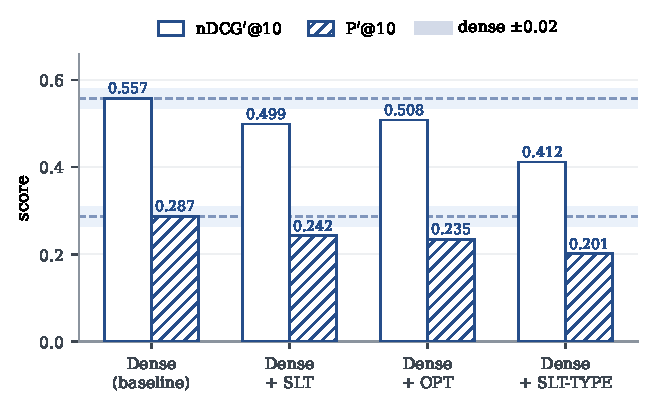
\includegraphics[width=0.78\textwidth]{images/ret_h11_add_one.pdf}
\caption[Adding one formula index to dense retrieval]{Dense retrieval against each configuration that adds one formula index to it. The
dashed lines mark dense retrieval's score and the bands the 0.02 resolving-power limit of
Section~\ref{sec:met-judge-validation}, within which two scores are indistinguishable. ARQMath-3
answer retrieval, the 78 official topics of Section~\ref{sec:met-collection}, judge-pool labels.
\emph{SLT}: symbol layout tree. \emph{OPT}: operator tree. \emph{SLT-TYPE}: the symbol layout
tree with its values erased. \emph{nDCG$'$@10}: prime normalised discounted cumulative gain at
rank 10. \emph{P$'$@10}: prime precision at rank 10.}
\label{fig:res-add-one}
\end{figure}

% --------------------------------------------------------------------------------------------
\subsection{Adding all three formula indexes}\label{sec:res-add-three}

Each of the three representations reads a formula differently. A symbol layout tree records how
it is written, an operator tree what it computes, and SLT-TYPE its shape with the values gone,
so an answer that one of them misses may be one another finds. Three rankings that fail on
different queries could cover for each other in a way no single pair can. Hypothesis H1.2
states that expectation in two clauses: the three-index system improves on the strongest
text-only retrieval, and it improves on adding one. The system it names is dense retrieval with
SLT, OPT and SLT-TYPE, each ranking entering the fusion on its own; how they enter is held
fixed here and varied in Section~\ref{sec:res-fusion}, so that one thing changes at a time.
Both clauses must hold on nDCG$'$@10 and P$'$@10, each gap beyond 0.02.

The first clause fails, and not narrowly (Figure~\ref{fig:res-add-three}). The four-ranking
system reaches 0.322 nDCG$'$@10 and 0.124 P$'$@10, against dense retrieval's 0.557 and 0.287.
It is 0.235 behind on the first measure and 0.163 behind on the second, eight times the limit
in each case.

The second fails with it. Against the highest of the three pairs of
Section~\ref{sec:res-add-one}, dense retrieval with OPT at 0.508 and 0.235, the four-ranking
system is 0.186 and 0.111 behind. Adding three formula rankings therefore leaves the system
further back than adding one did, and adding one had already left it behind dense retrieval
alone. More formula evidence makes the result worse, not better, and the fusion rule is a
candidate explanation: reciprocal rank fusion gives the top of every ranking the same weight
and has no way of knowing which ranking is the better one, as
Section~\ref{sec:bg-rank-fusion} sets out, so each formula ranking added is another vote of
equal standing.

Neither clause holds, and Section~\ref{sec:ret-verdicts} rules on H1.2. If the vote count is
what does the damage, then arranging the same three rankings so that they hold fewer votes
should undo some of it, and Section~\ref{sec:res-fusion} tests exactly that.

\begin{figure}[t]
\centering
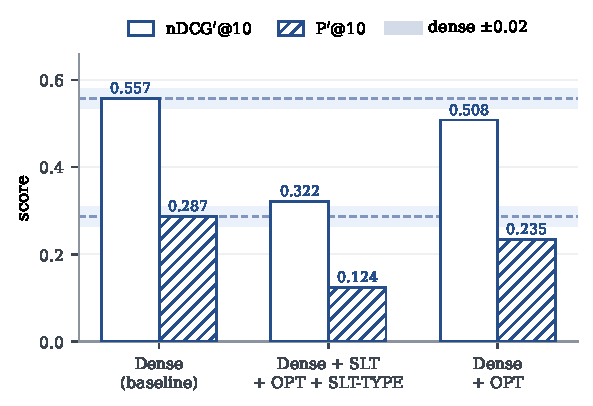
\includegraphics[width=0.70\textwidth]{images/ret_h12_add_all_three.pdf}
\caption[Adding all three formula indexes]{Dense retrieval against dense retrieval with all three formula rankings, each voting on
its own, and against the highest of the single-index configurations. The dashed lines mark dense
retrieval's score and the bands the 0.02 resolving-power limit of
Section~\ref{sec:met-judge-validation}. ARQMath-3 answer retrieval, the 78 official topics of
Section~\ref{sec:met-collection}, judge-pool labels. \emph{SLT}: symbol layout tree. \emph{OPT}:
operator tree. \emph{SLT-TYPE}: the symbol layout tree with its values erased.
\emph{nDCG$'$@10}: prime normalised discounted cumulative gain at rank 10. \emph{P$'$@10}: prime
precision at rank 10.}
\label{fig:res-add-three}
\end{figure}

% --------------------------------------------------------------------------------------------
\subsection{How the formula rankings enter the fusion}\label{sec:res-fusion}

The four-ranking system of Section~\ref{sec:res-add-three} gave each of the three formula
rankings a vote of its own. Nothing about those rankings, or about the fusion rule, is changed
here. Only the way they enter it is. Section~\ref{sec:met-retrieval-configs} fixed two arrangements
for that. The blocked system merges the three formula rankings into a single input before the
final fusion, so formula evidence holds one vote of three there. The flat system lets all five
rankings enter the final fusion directly, so formula evidence holds three votes of five.
Hypothesis H1.3 predicts that blocking beats flat fusion. The prediction rests on consistency:
blocking must be ahead in every cell of the comparison between the two full systems --- nDCG$'$
and P$'$ at 5, 10 and 20. Six cells, and one going the other way fails it.

Blocking is ahead in all six (Figure~\ref{fig:res-blocked-flat}). At nDCG$'$@10 the blocked
system reaches 0.551 against the flat system's 0.374. The margins run from 0.081 on P$'$@20 to
0.179 on nDCG$'$@20, every one of them clear of 0.02, and the ordering holds at every cutoff and
on both measures.

Blocking could work in either of two ways.

The first is that merging makes a better ranking. The three formula rankings fused with one
another might be stronger than any of them alone, in which case the final fusion is simply
receiving something better than it received before.

The second is that merging changes nothing about the formula evidence and only changes how many
votes it holds. Reciprocal rank fusion gives every input an equal vote, as
Section~\ref{sec:bg-rank-fusion} sets out, so the two vote counts above are the whole of the
difference between the arrangements. Every configuration in this chapter that took in formula evidence ended up below dense retrieval
alone. On this reading, then, blocking helps by letting less of that evidence through, not by
making it better.

Merging does improve the formula ranking on its own terms. Fused together, the three reach 0.261
nDCG$'$@10 (Table~\ref{tab:res-formula-block}), above SLT's 0.230 and OPT's 0.229 in
Table~\ref{tab:res-single-index} by more than 0.02. But no formula evidence is created by merging them. The flat system is given the
same three rankings, so whatever the merged ranking finds, the flat system's inputs find as
well. What separates the two arrangements is therefore not what the final fusion is shown. It is
how much of the final ranking that evidence is allowed to decide.

% [!ht], not [h]: bare [h] was promoted to [ht] on every build ("`h' float specifier changed to
%   `ht'" in the log).  The ! removes the warning and gives the float a fallback.
\begin{table}[!ht]
\centering
\small
\renewcommand{\arraystretch}{1.15}
\begin{tabular}{lrrrrrr}
\toprule
& \multicolumn{3}{c}{nDCG$'$} & \multicolumn{3}{c}{P$'$} \\
\cmidrule(lr){2-4}\cmidrule(lr){5-7}
Configuration & @5 & @10 & @20 & @5 & @10 & @20 \\
\midrule
Formula block & 0.244 & 0.261 & 0.285 & 0.100 & 0.091 & 0.078 \\
\bottomrule
\end{tabular}
\caption[The three formula rankings fused]{The three formula rankings fused with one another --- the \emph{formula block} ---
scored on its own. ARQMath-3 answer retrieval, the 78 official topics of
Section~\ref{sec:met-collection}, judge-pool labels; \emph{nDCG$'$} prime normalised discounted
cumulative gain and \emph{P$'$} prime precision, unjudged answers removed before scoring.}
\label{tab:res-formula-block}
\end{table}

The hole rates of Section~\ref{sec:ret-guards} show that weighting at work, since the text rankings return mostly answers the ARQMath assessors judged and the formula
rankings mostly answers they did not: 0.569 of the flat system's top ten carries no judgment,
against 0.238 of the blocked system's. With three votes of five the formula rankings fill much of
the flat list; with one vote of three they fill little of the blocked one.

Blocking beats flat fusion in every cell measured, which is what H1.3 predicted, and
Section~\ref{sec:ret-verdicts} rules on it. That formula evidence does less harm when it holds
fewer votes leaves one thing open: whether the harm is spread evenly across the three rankings
or concentrated in one of them. Section~\ref{sec:res-ablation} separates those.

\begin{figure}[t]
\centering
\definecolor{blockfill}{RGB}{233,233,233}
\resizebox{\textwidth}{!}{%
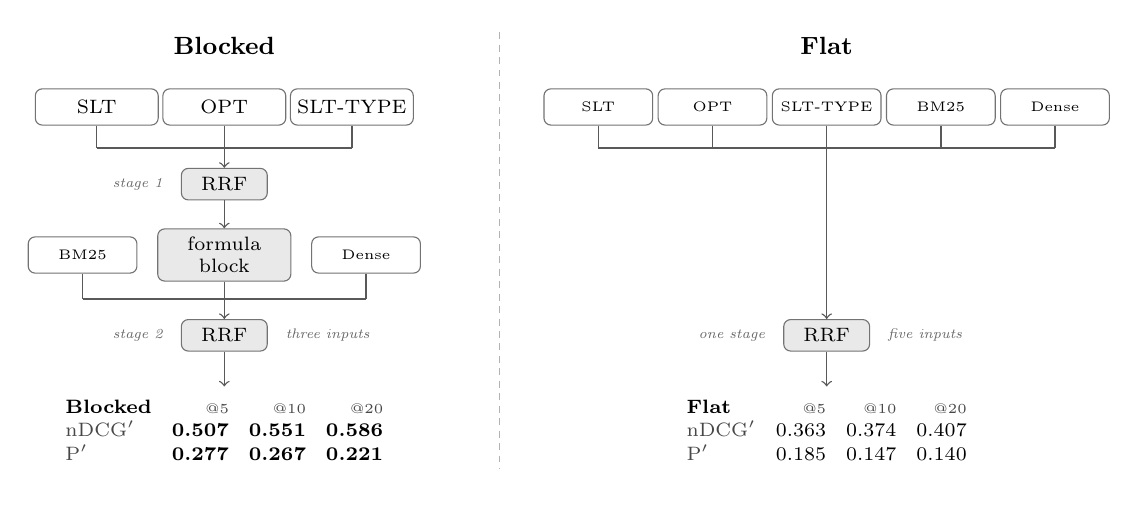
\begin{tikzpicture}[
  font=\scriptsize,
  card/.style={draw=black!55, rounded corners=2.5pt, fill=white, align=center,
               inner xsep=2pt, inner ysep=3pt, line width=0.4pt},
  idx/.style={card, text width=1.42cm, minimum height=0.46cm},
  nar/.style={card, text width=1.24cm, minimum height=0.46cm, font=\tiny},
  blk/.style={card, text width=1.55cm, minimum height=0.46cm, fill=blockfill},
  rrf/.style={card, text width=0.95cm, minimum height=0.40cm, fill=blockfill},
  flow/.style={->, draw=black!65, line width=0.5pt},
  wire/.style={draw=black!65, line width=0.5pt},
  stage/.style={font=\tiny\itshape, text=black!60},
]
\node[font=\small\bfseries] at (3.1,0.78) {Blocked};
\node[idx] (as) at (1.48,0) {SLT};
\node[idx] (ao) at (3.10,0) {OPT};
\node[idx] (at) at (4.72,0) {SLT-TYPE};
\foreach \n in {as,ao,at}{\draw[wire] (\n.south) -- (\n.south |- 0,-0.52);}
\draw[wire] (1.48,-0.52) -- (4.72,-0.52);
\node[rrf] (ar1) at (3.10,-0.98) {RRF};
\draw[flow] (3.10,-0.52) -- (ar1.north);
\node[stage, anchor=east] at ([xshift=-3pt]ar1.west) {stage 1};
\node[blk] (afb) at (3.10,-1.88) {formula block};
\draw[flow] (ar1.south) -- (afb.north);
\node[nar] (ab) at (1.30,-1.88) {BM25};
\node[nar] (ad) at (4.90,-1.88) {Dense};
\foreach \n in {ab,afb,ad}{\draw[wire] (\n.south) -- (\n.south |- 0,-2.44);}
\draw[wire] (1.30,-2.44) -- (4.90,-2.44);
\node[rrf] (ar2) at (3.10,-2.90) {RRF};
\draw[flow] (3.10,-2.44) -- (ar2.north);
\node[stage, anchor=east] at ([xshift=-3pt]ar2.west) {stage 2};
\node[stage, anchor=west, align=left] at ([xshift=3pt]ar2.east) {three inputs};
\node[anchor=north] (av) at (3.10,-3.55)
  {\setlength{\tabcolsep}{3.6pt}\renewcommand{\arraystretch}{1.08}%
   \begin{tabular}{@{}l r r r@{}}
   \toprule
   \textbf{Blocked} & {\color{black!72}\tiny @5} & {\color{black!72}\tiny @10}
     & {\color{black!72}\tiny @20}\\
   \midrule
   {\color{black!72}nDCG$'$} & \textbf{0.507} & \textbf{0.551} & \textbf{0.586}\\
   {\color{black!72}P$'$}    & \textbf{0.277} & \textbf{0.267} & \textbf{0.221}\\
   \bottomrule
   \end{tabular}};
\draw[flow] (ar2.south) -- (av.north);
\draw[black!30, dash pattern=on 2.5pt off 2pt, line width=0.4pt] (6.60,0.95) -- (6.60,-4.6);
\node[font=\small\bfseries] at (10.75,0.78) {Flat};
\node[nar] (bs) at (7.85,0)  {SLT};
\node[nar] (bo) at (9.30,0)  {OPT};
\node[nar] (bt) at (10.75,0) {SLT-TYPE};
\node[nar] (bb) at (12.20,0) {BM25};
\node[nar] (bd) at (13.65,0) {Dense};
\foreach \n in {bs,bo,bt,bb,bd}{\draw[wire] (\n.south) -- (\n.south |- 0,-0.52);}
\draw[wire] (7.85,-0.52) -- (13.65,-0.52);
\node[rrf] (br) at (10.75,-2.90) {RRF};
\draw[flow] (10.75,-0.52) -- (br.north);
\node[stage, anchor=east] at ([xshift=-3pt]br.west) {one stage};
\node[stage, anchor=west, align=left] at ([xshift=3pt]br.east) {five inputs};
\node[anchor=north] (bv) at (10.75,-3.55)
  {\setlength{\tabcolsep}{3.6pt}\renewcommand{\arraystretch}{1.08}%
   \begin{tabular}{@{}l r r r@{}}
   \toprule
   \textbf{Flat} & {\color{black!72}\tiny @5} & {\color{black!72}\tiny @10}
     & {\color{black!72}\tiny @20}\\
   \midrule
   {\color{black!72}nDCG$'$} & 0.363 & 0.374 & 0.407\\
   {\color{black!72}P$'$}    & 0.185 & 0.147 & 0.140\\
   \bottomrule
   \end{tabular}};
\draw[flow] (br.south) -- (bv.north);
\end{tikzpicture}}
\caption[Blocked against flat fusion]{Blocked against flat fusion. Both fuse the same five rankings and differ only in how the
three formula rankings enter: \emph{blocked} merges them into one input before the final fusion,
\emph{flat} lets all five enter it directly. Blocking is ahead in all six cells, by 0.081 to
0.179. ARQMath-3 answer retrieval, the 78 official topics of
Section~\ref{sec:met-collection}, judge-pool labels. \emph{RRF}: reciprocal rank fusion.
\emph{SLT}: symbol layout tree. \emph{OPT}: operator tree. \emph{SLT-TYPE}: the symbol layout
tree with its values erased. \emph{nDCG$'$}: prime normalised discounted cumulative gain.
\emph{P$'$}: prime precision.}
\label{fig:res-blocked-flat}
\end{figure}

% --------------------------------------------------------------------------------------------
\subsection{Removing an index}\label{sec:res-ablation}

If a weak ranking costs a fusion more than it contributes, taking it out should leave the fusion
better off. That runs against the assumption a multi-index system is built on, which is that each
index brings something the others do not. Hypothesis H1.4 predicts that every index
earns its place, so that removing any one of them makes the system worse. It is rejected
if any removal improves the system at nDCG$'$@10. Three ablations test it --- BM25 out of each
full system, and SLT-TYPE out of the flat fusion, which is the one arrangement where its ranking
holds a vote of its own.

Two removals behave as predicted (Table~\ref{tab:res-fusion-ablation}). Without BM25 the blocked
system falls from 0.551 to 0.522 at nDCG$'$@10 and the flat system from 0.374 to 0.322, both by
more than 0.02, so the weaker text index contributes to each of them despite what it scores
alone. The flat system is worse without BM25 in all six cells. The blocked system's loss shows on
nDCG$'$ at ranks 10 and 20; in the remaining four cells the two are indistinguishable.

The third runs the other way. Without SLT-TYPE the flat fusion rises from 0.374 to 0.416 at
nDCG$'$@10, and the gain clears 0.02 in five of six cells, the exception being P$'$@5 at 0.015.
SLT-TYPE was last of the five indexes on its own in
Section~\ref{sec:res-single-index}, and the fusion is better off without it. Under a rule that weights every ranking's top positions alike whatever that ranking
is worth, a weak index does not merely fail to help; it pushes better candidates down the fused
list.

One index is therefore not earning its place, and Section~\ref{sec:ret-verdicts} rules on H1.4.
The removal does not explain the whole of Section~\ref{sec:res-fusion}'s gap, though: without
SLT-TYPE the flat system reaches 0.416 and stays below the blocked system's 0.551 in all six
cells, by 0.059 to 0.137, even though the blocked system still contains SLT-TYPE.

What none of these comparisons explains is why formula evidence should hurt the retrieval it is
added to. That is a question about the signal rather than about the fusion, and
Section~\ref{sec:res-transfer} takes it up by looking at where a topic's formulas actually sit.

\begin{table}[t]
\centering
\small
\renewcommand{\arraystretch}{1.15}
\begin{tabular}{lrrrrrr}
\toprule
& \multicolumn{3}{c}{nDCG$'$} & \multicolumn{3}{c}{P$'$} \\
\cmidrule(lr){2-4}\cmidrule(lr){5-7}
Configuration & @5 & @10 & @20 & @5 & @10 & @20 \\
\midrule
Blocked                  & 0.507 & \textbf{0.551} & \textbf{0.586} & 0.277 & 0.267 & 0.221 \\
Blocked, $-$\,BM25       & 0.510 & 0.522 & 0.551 & 0.297 & 0.256 & 0.214 \\
\addlinespace
Flat                     & 0.363 & 0.374 & 0.407 & 0.185 & 0.147 & 0.140 \\
Flat, $-$\,BM25          & 0.313 & 0.322 & 0.349 & 0.151 & 0.124 & 0.109 \\
Flat, $-$\,SLT-TYPE      & 0.407 & 0.416 & 0.449 & 0.200 & 0.183 & 0.162 \\
\bottomrule
\end{tabular}
\caption[Removing one index from each full system]{The two full systems and the three configurations that remove one index from them, the
removed index marked by a leading minus. \emph{Blocked}: the three formula rankings merged into
one input. \emph{Flat}: each entering the fusion on its own. ARQMath-3 answer retrieval, the 78
official topics of Section~\ref{sec:met-collection}, judge-pool labels. \emph{SLT-TYPE}: the
symbol layout tree with its values erased. \emph{nDCG$'$}: prime normalised discounted cumulative
gain. \emph{P$'$}: prime precision. Where the two leading configurations differ by more than the
0.02 resolving-power limit of Section~\ref{sec:met-judge-validation}, the higher value is set in
bold; in the remaining four columns they are indistinguishable and neither is marked.}
\label{tab:res-fusion-ablation}
\end{table}


% §5.5 WHERE THE FORMULA SIGNAL LIVES -- rewritten 2026-09-25 (manifest §15 O-21 ii).
% The containment diagnostic.  It EXPLAINS §5.4's result rather than guarding an assumption, so it
%   follows the result and never precedes it, and it rules on nothing -- said plainly in its first
%   paragraph.  One page, no internal headings (manifest §9 row 5.5).
% It reads the ASSESSORS' labels directly and computes no retrieval measure, so §1c-i decision 2 --
%   one reporting channel in the results -- is untouched; §5.2.3's closing paragraph names it as
%   that site.
% Numbers, ALL from results/rearranged/formula_overlap_r7/overlap_summary.csv and
%   overlap_by_topic.csv, fanout, relevance = H+M, 78 official topics (manifest §14 R7):
%   OPT means 0.377 / 0.238 / 0.095 over all answers and 0.829 / 0.719 / 0.402 for the single best;
%   lead counts 70/78 then 30/78; at the maximum, 13 topics behind and 35 exactly tied (the 48 of
%   §5.4.5's RRF paragraph, split into its two parts); SLT 70 then 30, SLT-TYPE 72 then 17.
% tab:res-overlap RETIRED and replaced by fig:res-containment, OPT alone (Abram, 2026-09-25: nine
%   rows by eight columns asked the reader to derive the finding).  The other two representations
%   are carried in one sentence.  Figure from experiments/diagnostics/plot_containment_figure.py,
%   palette matched to the chapter's two other figures.
% NOT here: any hypothesis ID, clause or decision rule; any ratio (§1c-i decision 1); "channel"; a
%   containment redefinition of SLT-TYPE; the per-topic complete-match counts (47 / 34 / 32), which
%   the 35 ties already carry.
\section{Where the formula signal lives}\label{sec:res-transfer}

Section~\ref{sec:ret-guards} measured the formula block on the task its design was aimed at,
formula search, and found it performing comparably with a published system.
Section~\ref{sec:ret-results} measured the same three representations on answer retrieval, and
every configuration they joined scored below the text retrieval they were added to. The index
is not broken and the fusion is not misarranged; what changes between the two results is what
the task counts as relevant. This section takes that up. It decides no hypothesis, and explains
a result Section~\ref{sec:ret-results} has already established.

Nothing is retrieved for this measurement. It reads the organisers' judgments for the 78
official topics of Section~\ref{sec:met-collection} directly, the assessors' labels rather than
the judge's, since the question is what the assessors counted as relevant. Every formula on
both sides is converted to the tuples of Section~\ref{sec:met-formula-indexing}, and a pair of
formulas, one from the topic and one from an answer, is scored by \emph{containment}: the
fraction of the topic formula's tuples that appear in the answer's, so that one is a complete
match. The best-matching pair is kept for each answer, and the topic's formulas are selected by
the fanout of Section~\ref{sec:met-retrieval-configs}, so that what is measured is what the
formula indexes are given.

Relevant answers are compared against two controls, a hard one and an easy one, each matched in
number to the topic's relevant set. The hard control is the non-relevant judged answers of the
same topic, which isolates relevance from mere topical similarity. The easy control is answers
drawn at random from the collection. A topic's per-answer containment values are then collapsed
three ways: the mean over all answers, the mean of the top five, and the single best answer.
This shows how the signal behaves as the group narrows. The narrow end is the end an evaluation
measure reads, since nDCG$'$@10 and P$'$@10 see only the first few answers a ranking returns.

\begin{figure}[t]
\centering
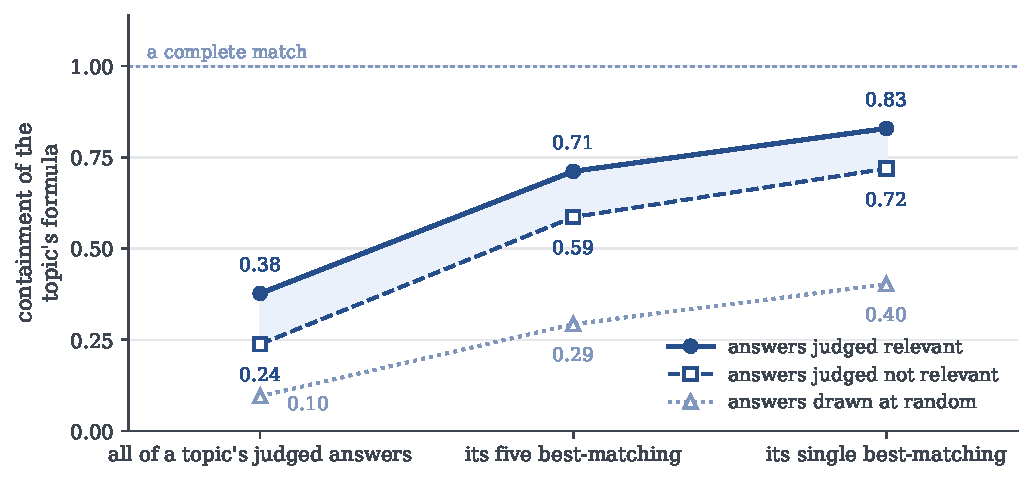
\includegraphics[width=0.92\textwidth]{images/res_containment_opt.pdf}
\caption[Containment of a topic's formulas]{Containment of a topic's formulas in its judged answers, under the \emph{OPT} (operator
tree) representation of Section~\ref{sec:met-formula-indexing}, over the 78 official topics of
Section~\ref{sec:met-collection} and scored against the organisers' own judgments.
\emph{Containment}: the fraction of a topic formula's path tuples that also appear in an
answer's formula, so that 1.00 is a complete match. Each point is a mean over the 78 topics, and
the three columns narrow the answers a topic contributes, from all of its judged answers to the
single one that matches best. The non-relevant and random groups are matched in number to the
topic's relevant set.}
\label{fig:res-containment}
\end{figure}

Averaged over all of a topic's answers, containment separates the two classes
(Figure~\ref{fig:res-containment}). Relevant answers contain 0.377 of the query formula's OPT
tuples against 0.238 for the same topic's non-relevant answers and 0.095 for random ones, and
they lead the hard control on 70 of the 78 topics. Those non-relevant answers were read against
this question and rejected, so they are about it too, and they still contain less of its
formulas. Being about the question is not what produces the difference. Narrow the group and the
separation erodes at every step: at the single best-matching answer relevant answers reach 0.829
against 0.719, and the lead falls to 30 topics, on 13 of which the non-relevant answer contains
more and on 35 of which the two are exactly equal. SLT behaves as OPT does, and SLT-TYPE
separates worst of the three at the narrow end, leading on 17.

This is why formula retrieval under fanout cannot match retrieval over text. Fanout queries with
every non-trivial formula in the topic, so almost every plausible candidate scores highly and
therefore scores alike: the right neighbourhood is retrieved, and nothing is left with which to
rank inside it. The relevance criteria then work against the index. A post that only restates the
question is non-relevant by definition (Section~\ref{sec:bg-arqmath}). A restatement carries the
question's formulas verbatim. So the closest structural match a formula index can find is often
the answer the criteria reject. Formula search grades the other way: its top level is calibrated
against exact structural match, which is close to what containment measures. The words around a
formula still separate an answer that derives a result from a comment that restates the question
using the same expression, and that is what the text rankings read.
Section~\ref{sec:ret-verdicts} takes this up with the results.


% §5.6 WHAT THIS SETTLES ABOUT RQ1 -- rewritten 2026-09-25 (manifest §15 O-20 c, d and O-21 iii).
% Rules on H1.1-H1.4 (the 2026-09-24 set, manifest §1c) in §5.4's order, one to one with
%   §5.4.3-§5.4.6: H1.1 not supported, H1.2 not supported (both clauses), H1.3 supported, H1.4 not
%   supported.  §5.3's component guard and §5.5's diagnostic rule on nothing and are read as
%   EVIDENCE in the closing paragraph, never as rulings (manifest §9 row 5.5).
% Verdict words are "supported" and "not supported" only -- the three-point scale was dropped
%   2026-09-25.  H1.1's partial grade never fires on these numbers (none of the three pairs is
%   ahead), so removing it cannot turn a fail into a pass and no disclosure is owed; §5.4.3 and
%   manifest §1c were edited the same day to match.
% THE BEST MULTI-INDEX RETRIEVER IS NAMED HERE, not in §6.1 (Abram, 2026-09-25): the selection is
%   made by reading RQ1's results, so it is a Chapter 5 outcome and §6.1 recaps it.  Blocked at
%   0.551 ndcg'@10 is the highest of every configuration built from more than one index -- ahead of
%   flat (0.374), of blocked without BM25 (0.522) and of BM25 + dense (0.539) -- so §1b's selection
%   rule resolves to it however tightly "multi-index" is read.
% Numbers, all from results/rearranged/ on the 78 official topics under the judge pool (§14):
%   dense 0.557 / 0.287 and BM25 + dense 0.539, metrics_judge_pool20 (R1.2, R3.1); dense + OPT
%   0.508 / 0.235, dense + SLT 0.499 / 0.242, dense + SLT-TYPE 0.412 / 0.201 (R3.2-R3.4); the three
%   formula rankings voting separately 0.322 / 0.124 (R3.9, H1.2's subject); blocked 0.551 / 0.267,
%   flat 0.374, blocked -BM25 0.522, flat -SLT-TYPE 0.416 (R3.6-R3.8, R3.10); blocked-flat margins
%   0.081-0.179; containment leads 70 then 30 topics (R7, OPT, fanout, H+M).
% NOT here: "Transfer" as a lead-in (the transfer question was dropped 2026-09-24); any bare task
%   number; "significant", "reliable", "dominates", any ratio, or any sentence saying which of
%   RQ1.2's two combination factors matters more (§1c-i decision 1); "channel"; any definition; a
%   hypothesis ID or a verdict in a heading or lead-in; any post-hoc disclosure -- H1.3's
%   restatement rests on §7.2's row alone (manifest §15 O-19 g).
% WARNING carried forward: §5.6 no longer states that dense retrieval IS the strongest text-only
%   retrieval.  §5.4.2 is now the ONLY site that does -- re-check it before Chapter 6 reads it.
\section{What this settles about RQ1}\label{sec:ret-verdicts}

Section~\ref{sec:ret-results} ran five experiments, and four of them decide a hypothesis. Formula
evidence that holds up at formula search adds nothing to answer retrieval that a dense retriever
has not already found. More of it makes the result worse rather than better. The arrangement that
lets the least of it through is the best system this chapter builds.

\textbf{Adding one formula index.} H1.1 predicted that each formula index, added to the strongest
text-only retrieval, improves answer retrieval over that retrieval alone.
Section~\ref{sec:res-single-index} resolves that dense retrieval on its own scores 0.557
nDCG$'$@10 over the 78 official topics. None of the three pairs reaches it --- 0.508 with OPT, 0.499
with SLT and 0.412 with SLT-TYPE, and 0.235, 0.242 and 0.201 on P$'$@10 against 0.287 --- and all
six gaps are wider than 0.02 (Figure~\ref{fig:res-add-one}). H1.1 is not supported, and the answer
to RQ1.1 is no.

\textbf{Adding all three.} H1.2 predicted that adding all three formula indexes improves on the
strongest text-only retrieval, and improves on adding one. Dense retrieval with the three formula
rankings each voting on its own reaches 0.322 nDCG$'$@10 and 0.124 P$'$@10, behind dense retrieval
alone by 0.235 and 0.163 and behind the best of the pairs, dense retrieval with OPT, by 0.186 and
0.111 (Figure~\ref{fig:res-add-three}). Both clauses fail and H1.2 is not supported. Three formula
rankings leave the system further back than one did.

\textbf{How the formula rankings are merged.} H1.3 predicted that blocking beats flat fusion --- the
same five rankings, with formula evidence holding one vote of three rather than three of five.
Blocking is ahead in all six cells the rule reads, by 0.081 to 0.179, and at the primary measure
0.551 against 0.374 (Figure~\ref{fig:res-blocked-flat}). H1.3 is supported.

\textbf{Whether every index earns its place.} H1.4 predicted that every index contributes, so that
removing any one of them makes the fused system worse. Removing BM25 costs both full systems.
Removing SLT-TYPE lifts flat fusion from 0.374 to 0.416 nDCG$'$@10, past 0.02 there and in five of
the six cells (Table~\ref{tab:res-fusion-ablation}), so one index does not earn its place. The
reciprocal rank fusion of Section~\ref{sec:bg-rank-fusion} gives every input the same vote however
weak that input is: blocking limits how many votes the formula rankings hold, and removing SLT-TYPE
takes away the weakest of them. Blocking is supported, and the hypothesis that every index earns
its place is not. The two verdicts carry one finding: how the rankings are merged and which of them
are chosen both matter.

\textbf{The best multi-index retriever.} Among the configurations built from more than one index,
the blocked system is the highest at the primary measure, at 0.551 nDCG$'$@10: ahead of every flat
arrangement and of the blocked system without BM25 at 0.522. It is therefore the best multi-index
retriever this chapter produces, and it is the retriever Chapter~\ref{ch:generation} gives a
generator. It does not beat text-only retrieval. Against dense retrieval it differs by 0.006 on
nDCG$'$@10 and 0.020 on P$'$@10, neither past the 0.02 of Section~\ref{sec:met-judge-validation},
so the two are indistinguishable on both reported measures. Section~\ref{sec:res-fusion} shows what
brings it that close: with formula evidence holding one vote of three, less of it reaches the final
ranking. Blocking earns its place by keeping that evidence from doing harm, not by supplying what
the text rankings lack.

\textbf{RQ1 as a whole.} Adding structure-aware formula indexes to text-only retrieval does not
improve answer retrieval. One formula index leaves the system 0.049 to 0.145 behind dense retrieval
at the primary measure, depending on which one is added. All three, each voting on its own, leave
it 0.235 behind. Only the blocked arrangement of all five rankings draws level with dense
retrieval. How they are combined does govern the result, and it is the whole of what the fused
systems differ by. The failure is not a property of the index. Section~\ref{sec:ret-guards}
measured the same three representations at formula search, where they perform comparably with a
published system (Table~\ref{tab:guard-task2-placement}), and Section~\ref{sec:res-transfer}
located the difference in what each task counts as relevant: a topic's formulas are contained in
the answers the assessors judged relevant more than in those they judged not relevant, leading on
70 of the 78 topics, but among the best-matching answers, where a ranking is decided, that lead
falls to 30 (Figure~\ref{fig:res-containment}). Formula matching retrieves the right neighbourhood
and cannot order inside it, and answer retrieval is graded on whether a post resolves the question.

Chapter~\ref{ch:generation} asks whether retrieval differences of these sizes reach the answer a
generator writes. Between the multi-index retriever and dense retrieval the difference is too small
to resolve; between either of them and any formula representation on its own it is large.
